\documentclass[11pt,oneside,letterpaper]{article}

% graphicx package, useful for including eps and pdf graphics
\usepackage{graphicx}
\DeclareGraphicsExtensions{.pdf,.png,.jpg}

% basic packages
\usepackage{color} 
\usepackage{parskip}
\usepackage{float}

% text layout
\usepackage{geometry}
\geometry{textwidth=15cm} % 15.25cm for single-space, 16.25cm for double-space
\geometry{textheight=22cm} % 22cm for single-space, 22.5cm for double-space

% helps to keep figures from being orphaned on a page by themselves
\renewcommand{\topfraction}{0.85}
\renewcommand{\textfraction}{0.1}

% bold the 'Figure #' in the caption and separate it with a period
% Captions will be left justified
\usepackage[labelfont=bf,labelsep=period,font=small]{caption}

% review layout with double-spacing
%\usepackage{setspace} 
%\doublespacing
%\captionsetup{labelfont=bf,labelsep=period,font=doublespacing}

% cite package, to clean up citations in the main text. Do not remove.
\usepackage{cite}
%\renewcommand\citeleft{(}
%\renewcommand\citeright{)}
%\renewcommand\citeform[1]{\textsl{#1}}

% Remove brackets from numbering in list of References
\renewcommand\refname{\large References}
\makeatletter
\renewcommand{\@biblabel}[1]{\quad#1.}
\makeatother

\usepackage{authblk}
\renewcommand\Authands{ \& }
\renewcommand\Authfont{\normalsize \bf}
\renewcommand\Affilfont{\small \normalfont}

% comments
\usepackage{ulem}
\definecolor{purple}{rgb}{0.459,0.109,0.538}
\def\tb#1#2{\sout{#1} \textcolor{purple}{#2}} 
\def\tbc#1{\textcolor{purple}{[#1]}}



%%% TITLE %%%
\title{\vspace{1.0cm} \LARGE \bf fluB}

\author[1]{Gytis Dudas}
\author[1]{Trevor Bedford}
\author[1]{Samantha Lycett}
\author[1,2]{Andrew Rambaut}

\affil[1]{Institute of Evolutionary Biology, University of Edinburgh, Edinburgh, UK}
\affil[2]{Fogarty International Center, National Institutes of Health, Bethesda, MD, USA.}

\date{\today}

\begin{document}
\maketitle

\begin{abstract}

Influenza B viruses are increasingly being recognized as major contributors to morbidity attributed to seasonal influenza. Currently circulating influenza B isolates are known to belong to two antigenically distinct lineages (B/Victoria and B/Yamagata subtypes) on the basis of haemagglutinin inhibition (HI) assays. Frequent reassortment of the two subtypes has been noted in the past, but the effects of these reassortments have not been investigated in much detail.

\end{abstract}

\pagebreak


\section*{Introduction}
Seasonal influenza causes an estimated 250,000 to 500,000 deaths annually and is comprised of three species (influenza A, B and C) co-circulating in humans. Though lacking in antigenic diversity, influenza B viruses are increasingly being recognized as being an important economic burden \cite{paul-glezen2013}. In the 2012/2013 influenza season in Europe as many as 53\% of influenza sentinel surveillance samples tested positive for influenza B \cite{ECDC1213}. 

As members of \textit{Orthomyxoviridae}, all influenza viruses have segmented genomes, which allow viruses co-infecting the same cell to exchange segments (a process known as reassortment). Influenza A viruses are widely considered to be a major threat to human health worldwide due to the ability to cause pandemics in humans via reassortment of seasonal human and non-human influenza A strains. The only known persistent source of influenza B viruses are humans (and occasionaly seals \cite{osterhaus2000}) and thus the antigenic diversity of influenza B viruses is considered to be low. It has been suggested that influenza B viruses use a combination of reassortment and amino acid insertion-deletion to generate antigenic novelty.

Influenza B viruses are considered to be comprised of two antigenically distinct lineages - Victoria and Yamagata (referred to as Vic and Yam, respectively) which are named after the strains (B/Victoria/02/87 and B/Yamagata/16/88, respectively) with antigenically distinct haemagglutinin (HA) surface glycoproteins. The two HA lineages still co-circulate today and are thought to have shared a most recent common ancestor in xxxx. All other influenza B segments also show a split in xxxx (comment - our estimate \textit{circa} 1984, use a figure to show TMRCAs and rates for each segment?).


\section*{Methods}

\subsection*{Sequences and subtyping}
We compiled a dataset of 452 complete influenza B genomes from GISAID (comment - need acknowledgment tables). Each strain was subtyped (assigned to either Vic or Yam subtype) in each segment by making maximum likelihood trees and looking whether it fell within the subtree containing B/Victoria/02/87 or B/Yamagata/16/88 sequences with the exception of the NS segment (B/Victoria/02/87 was a reassortant and possessed a Yam lineage NS), where B/Norway/1/84 was considered as being representative of Victoria lineage.
Each strain was thus assigned 8 subtypes depending on the combination of lineages it belongs to in all trees (for example all segments except for NS in strain B/Victoria/02/87 belong to Vic lineage and can thus be represented as V,V,V,V,V,V,V,Y). Seven of these where then used as discrete states in each of the trees (e.g. PB1 tree had PB2, PA, HA, NP, NA, MP and NS as traits and V or Y as trait values) in BEAST (comment - reference BEAST). (comment - give figure with proportions of subtypes for each segment)

\subsection*{Building trees}
For each segment it was attempted to make 3 replicates with 200 million MCMC states (comment - only third replicates ran for that long) each under the HKY model of nucleotide substitutions, 3 codon partitions, robust counting (comment - reference robust counting)) under the GMRF Bayesian skyride demographic model (comment - reference skyride).
In addition we used "relaxed" tips (comment - \# of relaxed tips) for when the dates of isolation for strains were incomplete (i.e. when only year of isolation was available).
We inferred the ancestral subtypes of lineages in each segment by using discrete traits (asymmetric CTMC matrix with BSSVS (comment - cite Philippe)). Because the posterior set of trees are labelled, we can infer intersubtype reassortments whenever a trait transition is observed (i.e. Y to V or V to Y). In addition, by reconstructing the subtypes of all other genomic segments jointly we can infer co-reassortment events when trait transitions occur on the same nodes in each tree.
We use a measure of persistence which is defined as the ratio of distances (in units of time) between a reassortant node and its most recent tip and compare it to the mean of distances between all nodes and their respective most recent tips. If this statistic is below 1 a reassortment event is presumed to be disadvantageous, if it is above 1 it is presumed it is advantageous.


\subsection*{Building a consensus set of reassortment events}
We built a consensus set of reassortment events by going through each tree in the posterior set of trees, identifying trait changes which are indicators of reassortment (with a cutoff of 1989 to avoid including the initial split between Vic and Yam as a reassortment event), taking the persistence value as the time between the date of reassortment (assumed to have occurred somewhere along the branch connecting nodes with opposite trait values) and the date of the most recent tip descended from that node. This was repeated for all nodes on the tree and the values averaged to give the average persistence time of nodes in the tree. We also noted which tips were descended from reassortant nodes.

We combined this list of reassortant clades across all posterior sets of segment trees based on descendant tips. There were a total of 3321 unique reassortant clades observed across all sets of posterior trees (comment - need a graph to show that most of the probability density is on a few well supported events or use different cutoffs?). By looking at only the nodes which occurred at least 20\% of the time in each tree and had a reassortment mapping that was found at least 50\% of the time, we recovered 29 "consensus" reassortment events.

\subsection*{Measure of diversity}
We inferred the diversity of each segment over time by taking the total distance between the most divergent branches on the tree at yearly intervals from 1986 to 2011. 

\subsection*{Work in progress}
Currently running "null" traited trees where trait maps have been rearranged (keeping the same ratio of trait values).

\section*{Results}


\begin{figure}[h]
	\centering		
	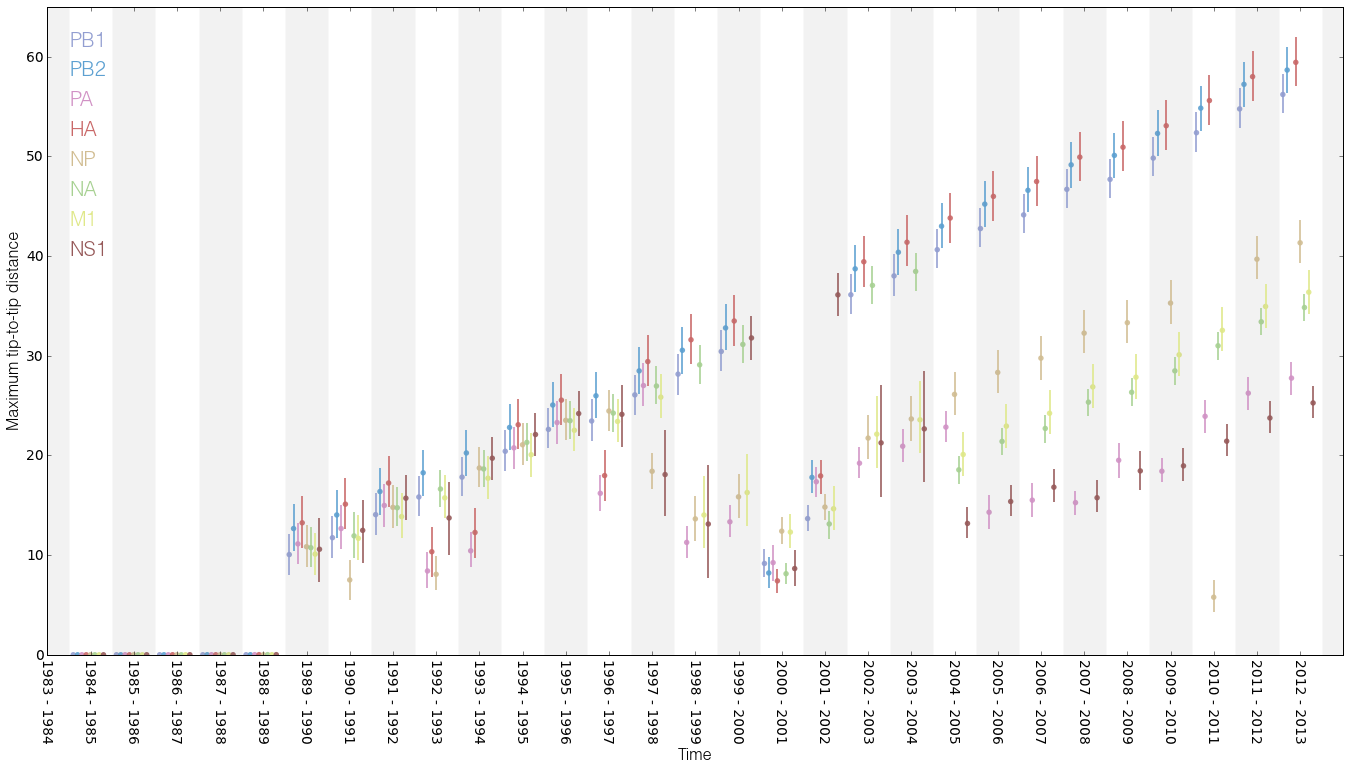
\includegraphics[width=0.95\textwidth]{figures/InfB_diversityOverTime}
	\caption{\textbf{Provisional diversity over time plot (tip to tip rather than branch to branch).}}
\end{figure}


\bibliographystyle{plos}
\bibliography{fluB}
\end{document}
